\documentclass{article}
\usepackage[utf8]{inputenc}
\usepackage{setspace}
\usepackage{amsmath}
\usepackage{enumerate}
\usepackage{enumitem}
\usepackage{moreenum}
\usepackage{multirow}
\usepackage[greek,english]{babel}
\usepackage{alphabeta}
\usepackage{tabularx}
\usepackage{graphicx}

\title{\textbf{Εργασία Στην Αριθμητική Ανάλυση}}
\author{\textbf{Ονοματεπώνυμο: Νικόλαος Βογιατζής} \\ \textbf{ΑΕΜ: 3952}}

\date{\textbf{Ημερομηνία Παράδοσης: 27/12/2022}}


\begin{document}
\maketitle
\textbf{Σημείώση:} Ο κώδικας που επιλύει την κάθε άσκηση υλοποιήθηκε στη γλώσσα προγραμματισμού της python\\
\par\textbf{\large{Άσκηση 1:}}\\
\par
\textbf{\large{Γραφική παράστασή της συνάρτησης:}}

\begin{equation*}
    f(x) =  e^{\sin^3x} + x^6 -2x^4 -x^3 -1
\end{equation*}

\begin{center}
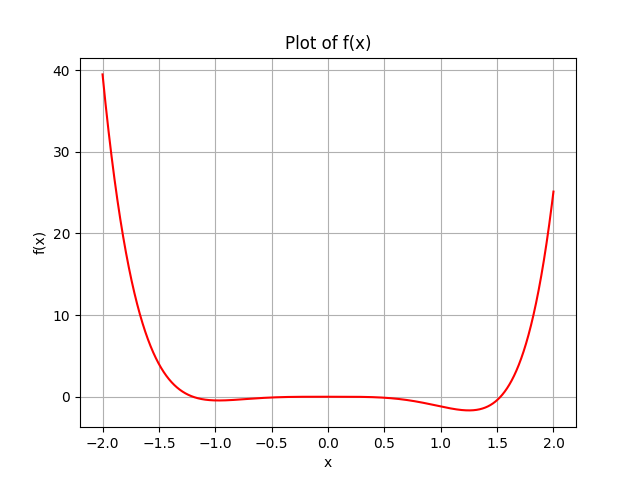
\includegraphics[width=.9\linewidth]{ex1_plot.png}
\end{center}
\newpage

\textbf{\large{Σημείωση:} } Ο κώδικας υλοποίησης της πρώτης άσκησης βρίσκεται στο αρχείο numanal2022ex1
\par\textbf{\large{Ερώτημα 1ο }:}
{Εύρεση ριζών με τη μέθοδο της διχοτόμησης, τη μέθοδο Newton-Raphson και τη μέθοδο της τέμνουσας στο διάστημα [-2,2] με ακρίβεια 5 δεκαδικών ψηφίων}\\
\par 
a)  Η συνάρτηση που υλοποιεί τον αλγόριθμο της \textbf{διχοτόμησης} δέχεται ως ορίσματα τα άκρα του διαστήματος [a,b] και το πλήθος των επαναλήψεων -n- που χρειάζονται για την προσέγγιση της ρίζας με ακρίβεια πέντε δεκαδικών ψηφίων. Εκτελείται μία λούπα n φορές όπου κάθε φορά υπολογίζεται το μέσο m του διαστήματος [a,b]. Ελέγχεται αν το μέσο είναι ρίζα της συνάρτησης f(x) ,οπότε και σταματά η λούπα. Διαφορετικά ελέγχεται αν η τιμή της συνάρτησης στο μέσο επί την τιμή του αριστερού άκρου του διαστήματος είναι μικρότερη του μηδενός \begin{equation*}
(f(m)f(a) < 0)\end{equation*}, όπου λαμβάνουμε ως νεό διάστημα εξέτασης το [a,m], ενώ σε κάθε άλλη περίπτωση λαμβάνουμε ως νέο διάστημα εξέτασης το [m,b]
\\
Ή εκτέλεση του αλγορίθμου 18 φορές, όπως βρίσκουμε σύμφωνα με τον τύπο 
\begin{equation*}
    N > \frac{\log(b-a) - \log(error)}{\log2}
\end{equation*}
όπου error = 0.000005 αφού μιλάμε για ακρίβεια πέντε δεκαδικών ψηφίων μας δίνει τις ρίζες a) -1.19762 , b)1.53013
. Για την ρίζα a) επιλέγουμε ως αρχικό διάστημα το [-2, -0.5] αφού διαπιστώσουμε πως 
\begin{equation*}
(f(a)f(b) < 0)\end{equation*} άρα μπορούμε να αναζητήσουμε και ρίζα. Αντίστοιχα εργαζόμαστε και για το αρχικό διάστημα της δεύτερης ρίζας το οποίο είναι το [0.5, 2]\\
\par
b) Η συνάρτηση υλοποίησης του αλγορίθμου \textbf{Newton-Raphson} δέχεται ως όρισμα την αρχική εκτίμηση της ρίζας x. Καταχωρεί σε μία μεταβλητή error το πηλίκο $f(x)$/$f'(x)$. Όσο αυτή η τιμή error είναι μεγαλύτερη ή ίση απο 0.000005 , ώστε να πετύχουμε την ακρίβεια των πέντε δεκαδικών ψηφίων στην εκτίμηση της ρίζας, εκτελείται μία λούπα στην οποία υπολογίζεται εκ νέου η τιμή της μεταβλητής error και πλέον η νέα τιμή της προσέγγισης της ρίζας x, είναι η παλιά μείον του σφάλματος error (x = x-error). Η επιλογή της συνθήκης τερματισμού της λούπας έγινε έτσι ώστε αν η τιμή $f(x)$ / $f'(x)$ τείνει πολύ κοντά στο μηδέν, φτάσει δηλαδή ή ξεπεράσει το 0.000005 η τιμή του x είναι πλέον η τιμή της ρίζας που ψάχνουμε. Η συνάρτηση επιστρέφει την εκτίμηση της ρίζας και μία μεταβλητή που δείχνει το πλήθος των επαναλήψεων που χρειάστηκαν για την εκτίμηση της ρίζας για τη δοθείσα ακρίβεια. 
Η αρχική εκτίμηση της ρίζας επιλέχθηκε έτσι ώστε να ισχύει $f(x)$ $f''(x)>0$
Για την πρώτη ρίζα επιλέγουμε ως αρχική εκτίμηση το -2, εφόσον ισχύει η παραπάνω συνθήκη και βρίσκουμε έπειτα από 11 επαναλήψεις το -1.19762.\\ Για τη δεύτερη ρίζα επιλέγουμε ως αρχική εκτίμηση το 2 κι έπειτα απο 7 επαναλήψεις βρίσκουμε το 1.53013
\par 
c)  Η συνάρτηση που υλοποιεί τη μέθοδο της \textbf{τέμνουσας} δέχεται δύο ορίσματα x0 και x1 , τα οποία αποτελούν τις δύο αρχικές συνθήκες
Για την εύρεση της ρίζας τρέχει ένας ατέρμων βρόχος στον οποίο υπολογίζεται η τιμή error η οποία είναι ίση με $(x1 - x0) *f(x0)/(f(x1)-f(x0))$ . Η νέα εκτίμηση για τη ρίζα είναι η x2 = x0 - error και οι πλέον αρχικές συνθήκες οι x0 = x1 και x1 = x2. Η λούπα σταματά όταν η τιμή του error γίνει μικρότερη από 0.000005, αφού αναζητούμε ρίζα με ακρίβεια 5 δεκαδικών ψηφίων. Όταν η παραπάνω συνθήκη γίνει αληθής γνωρίζουμε πλέον ότι η τιμή x1 αποτελεί τη ρίζα μας με την επιθυμητή ακρίβεια.
\par Για την εύρεση της πρώτης ρίζας επιλέγουμε ως αρχικά σημεία τα 
x0 = -1.5 και x1 = -1 κι έπειτα από 12 επαναλήψεις βρίσκουμε τη ρίζα -1.19762, ενώ για τη δεύτερη ρίζα με αρχικές συνθήκες τα x0 = 1.2 και x1 = 2 έπειτα απο 20 επαναλήψεις βρίσκουμε τη ρίζα 1.53013\\

\newpage
\textbf{\large{Άσκηση 2:}}\\
\par
\textbf{\large{Γραφική παράστασή της συνάρτησης:}}

\begin{equation*}
    f(x) = 94cos^3x - 24cosx + 177sin^2x - 108sin^4x - 72cos^3xsin^2x -65
\end{equation*}
\begin{center}
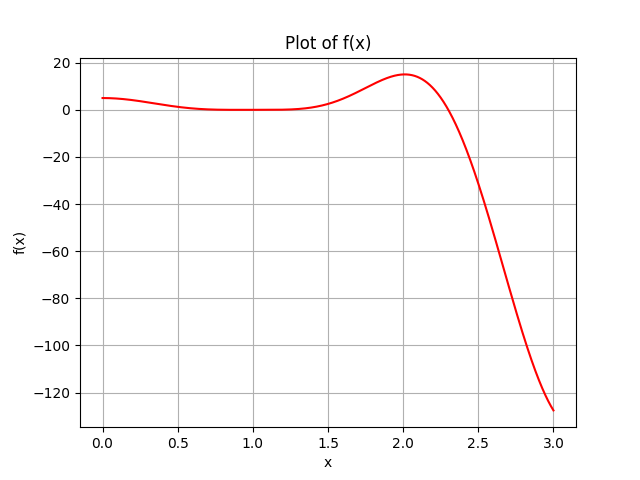
\includegraphics[width=.9\linewidth]{ex2_plot.png}
\end{center}

\textbf{\large{Σημείωση: } } Ο κώδικας της δεύτερης άσκησης βρίσκεται στο αρχείο ex2numanal2022
\par\textbf{\large{Ερώτημα 1ο }:}
{Εύρεση ριζών με τις τροποποιημένες μεθόδους της \textbf{διχοτόμησης}, \textbf{newton-raphson} και \textbf{τέμνουσας} στο διάστημα [0, 3] με ακρίβεια 5 δεκαδικών ψηφίων}
\par Με την τροποποιημένη μέθοδο της διχοτόμησης βρίσκουμε:
\begin{itemize}
\item ρίζα 1η: 0.84107 σε $\approx$26 επαναλήψεις με αρχικό διάστημα [0,1]
\item ρίζα 2η: 1.04719 σε $\approx$27 επαναλήψεις με αρχικό διάστημα [1,2]
\item ρίζα 3η: 2.30052 σε $\approx$30 επαναλήψεις με αρχικό διάστημα [2,3]
\end{itemize}
 Η συνθήκη τερματισμού της επανάληψης (όπου αναζητούμε ρίζα με την δοθείσα ακρίβεια) είναι η διαφορά του δεξιού απο του αριστερόυ άκρου του διαστήματος σε απόλυτη τιμή να γίνει μικρότερη του 0.000005 ($abs(b-a)<0.000005$, ενώ η επιλογή της νέας ρίζας κάθε φορά γίνεται με την αρχικοποίηση ενός τυχαίου αριθμού εντός των άκρων.
 \newpage
\parΜε την τοποποιημένη μέθοδο \textbf{newton-raphson} βρίσκουμε:
\begin{itemize}
\item ρίζα 1η: 0.84107 σε 11 επαναλήψεις με αρχική τιμή x0 = 0.2
\item ρίζα 2η: 1.04850 σε 254 επαναλήψεις με αρχική τιμή x0 = 1.5
\item ρίζα 3η: 2.30052 σε 4 επαναλήψεις με αρχική τιμή x0 = 2.5
\end{itemize}

Η τροποποιημένη μέθοδος newton-raphson λειτουργεί παρόμοια με την γνήσια μέθοδο, με τη μόνη αλλαγή πως η συνθήκη τερματισμού της επανάληψης έιναι πλέον η τιμή error να γίνει μικρότερη από 0.000005,όπου
\begin{center}error = 1/(($f'(xn)$ / $f(xn)$) - ($f''(xn)$ / $2f'(xn)$))\end{center}
και  η προηγούμενη προσέγγιση της ρίζας.

\par  Με την τροποποιημένη μέθοδο της τέμνουσας βρίσκουμε:
\begin{itemize}
    \item ρίζα 1η: 0.84107σε 12 επαναλήψεις με αρχικές συνθήκες x0 = 0, x1= 0.1  ,x2 = 0.5
    \item ρίζα 2η: 1.04718 σε 27 επαναλήψεις με αρχικές συνθήκες x0 = 1, x1= 1.5  ,x2 = 2\\
    \itemρίζα 3η: 2.30052 σε 7 επαναλήψεις με αρχικές συνθήκες x0 = 2, x1= 2.5  ,x2 = 3\\
\end{itemize}

\par \textbf{\large{Ερώτημα 2ο }:}
Εκτελούμε τον αλγόριθμο της τροποποιημένης διχοτόμησης για κάθε ρίζα που βρήκαμε απο το ερώτημα ένα 10 φορές και παίρνουμε τα παρακάτω αποτελέσματα:
\begin{center}
\begin{tabular}{|c||c|c|c|c|} 
 \hline
 Ρίζα & 0.84107 & 1.04719 & 2.30052 \\ [0.5ex] 
 \hline\hline
 Επαναλήψεις: & 30 & 39 & 28  \\ 
 \hline
 Επαναλήψεις: & 23 & 33 & 26 \\
 \hline
 Επαναλήψεις: & 22 & 21 & 25  \\
 \hline
 Επαναλήψεις: & 17 & 24 & 20 \\
 \hline
 Επαναλήψεις: & 25 & 21 & 22 \\ 
 \hline
 Επαναλήψεις: & 22 & 24 & 32\\
 \hline
 Επαναλήψεις: & 25 & 26 & 21 \\
 \hline
 Επαναλήψεις: & 21 & 27 & 27 \\
 \hline
 Επαναλήψεις: & 23 & 21 & 24 \\
 \hline
 Επαναλήψεις: & 25 & 17 & 25 \\[1ex] 
 \hline
\end{tabular}
\end{center}
Από τον παραπάνω πίνακα συμπεραίνουμε πως η τροποποιημένη μέθοδος της διχοτόμησης δεν συγκλίνει πάντα στον ίδιο αριθμό επαναλήψεων κι αυτό συμβαίνει καθώς δεν ορίζουμε τη προσέγγιση της ρίζας ως το μέσο του διαστήματος εξέτασης αλλά ως έναν τυχαίο αριθμό εντός του διαστήματος που εξετάζουμε\\
\par \textbf{\large{Ερώτημα 3ο }:}\\
Βρίσκουμε από κάθε μέθοδο μία ρίζα με τη γνήσια και την τροποποιημένη μέθοδο κάθε φορά και καταλήγουμε στα παρακάτω:
\begin{center}
\begin{tabular}{|c|c|c|c|} 
 \hline
 Ρίζα & 0.84107 & 1.04719 & 2.30052 \\ [0.5ex] 
 \hline\hline
  Newton-Raphson: & 7 & 29  & 5 \\ 
 \hline
 Τροποποιημένη:  & 11 & 254 & 4  \\[1ex]
 \hline
\end{tabular}
\end{center}
 \begin{center}
\begin{tabular}{|c|c|c|c|} 
 \hline
 Ρίζα & 0.84107 & 1.04719 & 2.30052 \\ [0.5ex] 
 \hline\hline
  Διχοτόμηση: & 17 & 16 & 18\\ 
 \hline
 Τροποποιημένη: & $\approx$25 & $\approx$30 & $\approx$ 25 \\[1ex]
 \hline
 \end{tabular}
 \end{center}
  \begin{center}
\begin{tabular}{|c|c|c|c|} 
 \hline
 Ρίζα  & 0.84107 & 1.04719 & 2.30052  \\ [0.5ex] 
 \hline\hline
    Τέμνουσα: &11 & 31 & 9  \\ 
 \hline
    Τροποποιημένη: &12 & 27 & 7  \\[1ex]
 \hline
\end{tabular}
 \end{center}
\parΒλέπουμε ότι τα αποτελέσματα δεν είναι ξεκάθαρα. Η κλασική μέθοδος της διχοτόμησης μόνο, φαίνται να παρουσιάζει γρηγορότερα αποτελέσματα από την τροποποιημένη κι αυτό συμβαίνει διότι για να προσεγγίσουμε τις ρίζες, εργαζόμαστε με μικρά διαστήματα οπότε το "σπάσιμο" των διαστημάτων στην μέση είναι ταχύτερο από το να αρχικοποιόυμε την νέα ρίζα με μία τυχαία τιμή (Μπορεί συχνά η γενήτρια τυχαίων τιμών να επιστρέφει μία τιμή πολύ κοντά σε κάποιο από τα άκρα του διαστήματος, οπότε και δε θα μικραίνει το διάστημα σημαντικά).
\parΗ κλασική μέθοδος Newton-Raphson θα μπορούσαμε να πούμε πως εμφανίζει καλύτερα αποτελέσματα από την τροποποιημένη. Οι δύο ρίζες προσεγγίστηκαν με σχεδόν ίδιο αριθμό επαναλήψεων ενώ βλέπουμε ότι η μία χρειάστηκε 220 - περίπου - επαναλήψεις περισσότερες για την προσέγγιση της με την τροποποιημένη μέθοδο από την κλασική.
\par Η κλασική μέθοδος της τέμνουσας θα λέγαμε ότι παρουσιάζει παρόμοια αποτελέσματα με αυτήν της τροποποιημένης μεθόδου.
\newpage
\textbf{\large{Άσκηση 3:}}\\
\textbf{Σημείωση: } Ο κώδικας της άσκησης 3 βρίσκεται στο αρχείο ex3numanal2022
\par\textbf{Ερώτημα 1ο:}
Οι πίνακες δημιουργήθηκαν ως λίστες λιστών. Για παράδειγμα ο πίνακας Α του παραδείγματος που χρησιμοποιήθηκε περιέχει σε μία λίστα τριών θέσεων μία λίστα τριών θέσεων σε κάθε θεση.Κάθε μία από τις εμφολευμένες λίστες αποτελεί μια γραμμή του πίνακα. \\Έτσι δημιουργείται ο πίνακας συντελεστών των αγνώστων Α = 
\begin{vmatrix}
 2 & 1 & 5\\
 4 & 4 & -4\\
 1 & 3 & 1\\
\end{vmatrix}\\
και ο πίνακας στήλη σταθερών όρων b = 
\begin{bmatrix}
5\\0\\6\\
\end{bmatrix}
Η εφαρμογή της παραγοντοποίησης PA = LU ,
δίνει τους παρακάτω πίνακες:\\
P = 
\begin{vmatrix}
 0 & 1 & 0 \\
 0 & 0 & 1\\
 1 & 0 & 0
\end{vmatrix},
Α = 
\begin{vmatrix}
 2 & 1 & 5\\
 4 & 4 & -4\\
 1 & 3 & 1
\end{vmatrix}
 = 
 L = 
 \begin{vmatrix}
 1 & 0 & 0\\
 0.25 & 1 & 0\\
 0.5 & -0.5 & 1
\end{vmatrix}
U = 
\begin{vmatrix}
 4 & 4 & -4\\
 0 & 2 & 2\\
 0 & 0 & 8
\end{vmatrix}\\
Αφού έχει επιτευχθεί η παραγοντοποίηση πρέπει να λυθούν δύο ακόμη συστήματα. Πρώτα το Lc = Pb ως προς c
κι έπειτα το  Ux = c ως προς x.
Εκτελώντας τα παραπάνω βήματα παίρνουμε στην έξοδο το διάνυσμα x = 
\begin{bmatrix}
-1\\2\\-1\\
\end{bmatrix}
που αποτελεί τη λύση του συστήματος. \\Σημείωση: Ο κώδικας δεν εξηγείται στο pdf αρχείο καθώς υπάρχουν αναλυτικά σχόλια στο αρχείο του κώδικα\\
\textbf{Ερώτημα 2ο:}
Για την παραγοντοποίηση Cholesky χρησιμοποιήθηκε ο πίνακας 
\begin{center}
Α = 
\begin{vmatrix}
 4 & -2 & 2\\
 -2 & 2 & 4\\
 2 & -4 & 11
\end{vmatrix}\\
\end{center}
Δημιουργούμε αρχικά τον πίνακα Α. Έπειτα τον εισάγουμε ως όρισμα στην συνάρτηση cholesky(A), και τον αντιγράφουμε σε έναν πίνακα Χ ίδιων διαστάσεων. Σε μία λούπα για όλες τις γραμμές του πίνακα Χ, εκτελούμε άλλη μία λούπα για όλες τις στήλες του πίνακα Χ. Μέσα στη δεύτερη λούπα, εργαζόμαστε ως εξής: Για τα στοιχεία της διαγωνίου βρίσκουμε την τιμή που θα πάρει ο κάτω τριγωνικός πίνακας για το διαγώνιο στοιχείο ,μέσα σε μία λούπα , που εξετάζουμε σύμφωνα με τον τύπο:
\begin{equation*}
   L_{j,j}=\sqrt{A_{i,j}- \sum_{k=1}^{j-1} L^2_{j,k}}
\end{equation*}
\\, ενώ για τα στοιχεία που δεν ανήκουν στη διαγώνιο εργαζόμαστε σε μία λούπα με τον τύπο:
\begin{equation*}
     L_{i,j} = \frac{1}{L_{j,j}}({A_{i,j} - \sum_{k=1}^{j-1} L_{i,k}L_{j,k}})
\end{equation*}\\
Για την επαλήθευση της εγκυρότητας της μεθόδου της αποσύνθεσης Cholesky, ορίζουμε έναν πίνακα $L^Τ$ που είναι ο ανάστροφος του κάτω τριγωνικού πίνακα L,  δηλαδή ένας άνω τριγωνικός πίνακας με γραμμές τις στήλες του πίνακα L και στήλες τις γραμμές του πίνακα L. Αν λοιπόν πολλαπλασιάσουμε τον πίνακα L με τον πίνακα $L^T$ παίρνουμε ως αποτέλεσμα τον αρχικό πίνακα A\\
\textbf{Ερώτημα 3ο:}
\par Για τη μέθοδο GaussSeidel αρχικοποιούμε τον πίνακα στήλη b = $[3,1,1,1,1,1,1,1,1,3]^T$ τον αραιό πίνακα 10*10 \\Α = 
\begin{vmatrix}
 5 & -2 & 0 & 0 & 0 & 0 & 0 & 0 & 0 & 0\\
 -2 & 5 & -2 & 0 & 0 & 0 & 0 & 0 & 0 & 0\\
 0 & -2 & 5 & -2 & 0 & 0 & 0 & 0 & 0 & 0\\
 0 & 0 & -2 & 5 & -2 & 0 & 0 & 0 & 0 & 0\\
 0 & 0 & 0 & -2 & 5 & -2 & 0 & 0 & 0 & 0\\
 0 & 0 & 0 & 0 & -2 & 5 & -2 & 0 & 0 & 0\\
 0 & 0 & 0 & 0 & 0 & -2 & 5 & -2 & 0 & 0\\
 0 & 0 & 0 & 0 & 0 & 0 & -2 & 5 & -2 & 0\\
 0 & 0 & 0 & 0 & 0 & 0 & 0 & -2 & 5 & -2\\
 0 & 0 & 0 & 0 & 0 & 0 & 0 & 0 & -2 & 5\\
\end{vmatrix}\\


και εκτελούμε τον αλγόριθμο μέχρι η
διαφορά της άπειρης νόρμας της προσέγγισης από την άπειρη νόρμα της προηγούμενης προσέγγισης να γίνει μικρότερη ή ίση από 0.00005 (αφού θέλουμε ακρίβεια τεσσάρων δεκαδικών ψηφίων.
Δηλαδή 
\begin{equation*}
   {\parallel{xold - x}}\parallel_{\infty} \leq{0.00005}
\end{equation*}
ο πίνακας στήλη των τιμών x που παίρνουμε στην έξοδο έπειτα από 23 επαναλήψεις
είναι το παρακάτω\\ 
x = $[0.9999,0.9999,0.9999,0.9999,0.9999,0.9999,0.9999,0.9999,0.9999,0.9999]^T$
Ανάλογα εργαζόμαστε και για τον πίνακα 10.000*10.000

\newpage

\textbf{\large{Άσκηση 4: }}\\
\textbf{Σημειώση: } Ο κώδικας που επιλύει την άσκηση 4 βρίσκεται στο αρχείο numanal2022_ex4.py
\par
Στην άσκηση αυτή μας δίνεται ο πίνακας A $\in$ $\mathbb{R}^{nxn}$, όπου A[n][n], n=15 ο πίνακας γειτνίασης της σύνδεσης της ιστοσελίδας i με την ιστοσελίδα j \\
\begin{center}

\setcounter{MaxMatrixCols}{15}

\textbf{Α}=\begin{pmatrix}
0 & 1 & 0 & 0 & 0 & 0 & 0 & 0 & 1 & 0 & 0 & 0 & 0 & 0 & 0\\
0 & 0 & 1 & 0 & 1 & 0 & 1 & 0 & 0 & 0 & 0 & 0 & 0 & 0 & 0\\
0 & 1 & 0 & 0 & 0 & 1 & 0 & 1 & 0 & 0 & 0 & 0 & 0 & 0 & 0\\
0 & 0 & 1 & 0 & 0 & 0 & 0 & 0 & 0 & 0 & 0 & 1 & 0 & 0 & 0\\
1 & 0 & 0 & 0 & 0 & 0 & 0 & 0 & 0 & 1 & 0 & 0 & 0 & 0 & 0\\
0 & 0 & 0 & 0 & 0 & 0 & 0 & 0 & 0 & 1 & 1 & 0 & 0 & 0 & 0\\
0 & 0 & 0 & 0 & 0 & 0 & 0 & 0 & 0 & 1 & 1 & 0 & 0 & 0 & 0\\
0 & 0 & 0 & 1 & 0 & 0 & 0 & 0 & 0 & 0 & 1 & 0 & 0 & 0 & 0\\
0 & 0 & 0 & 0 & 1 & 1 & 0 & 0 & 0 & 1 & 0 & 0 & 0 & 0 & 0\\
0 & 0 & 0 & 0 & 0 & 0 & 0 & 0 & 0 & 0 & 0 & 0 & 1 & 0 & 0\\
0 & 0 & 0 & 0 & 0 & 0 & 0 & 0 & 0 & 0 & 0 & 0 & 0 & 0 & 1\\
0 & 0 & 0 & 0 & 0 & 0 & 1 & 1 & 0 & 0 & 1 & 0 & 0 & 0 & 0\\
0 & 0 & 0 & 0 & 0 & 0 & 0 & 0 & 1 & 0 & 0 & 0 & 0 & 1 & 0\\
0 & 0 & 0 & 0 & 0 & 0 & 0 & 0 & 0 & 1 & 1 & 0 & 1 & 0 & 1\\
0 & 0 & 0 & 0 & 0 & 0 & 0 & 0 & 0 & 0 & 0 & 1 & 0 & 1 & 0
\end{pmatrix}\\
    
\end{center}
\par Στον παραπάνω πίνακα το κάθε κελί είναι είτε 1 έιτε 0. Η σύνδεση είναι 1 όταν συνδέεται ο κόβος i με τον κόμβο j, αλλιώς είναι 0. Βάσει του παραπάνω πίνακα δημιουργείται και ο πίνακας Google σύμφωνα με τον τύπο: \\
\[G_{i,j}=\frac{q}{n}+\frac{A_{j,i}(1-q)}{n_j}\] \\
, όπου q είναι η πιθανότητα μετακίνησης του χρήστη σε μία τυχαία σελίδα (q = 0.15), 1-q ο χρήστης επιλέξει τυχαία έναν από τους συνδέσμους της σελίδας i, n το μέγεθος του πίνακα - εδώ n=15 - και nj ο πίνακας μεγέθους n με στοιχεία το άθροισμα της j-οστής γραμμής του πίνακα Α, δηλαδή το πλήθος συνδέσεων της σελίδας j.

\par\textbf{Ερώτημα 1ο: } Απόδειξη ότι ο πίνακας G (πίνακας Google) είναι στοχαστικός. Για να είναι ένας πίνακας στοχαστικός πρέπει το άθροισμα κάθε στήλης του πίνακα να έχει άθροισμα ίσο με το 1. Αρχικά, δημιουργήθηκε ο πίνακας Α, στον πίνακα nj μεγέθους 15 εισάγαμε σε κάθε θέση του το άθροισμα της j-οστής γραμμής του πίνακα Α κι έπειτα υπολογίστηκε το κάθε κελί του πίνακα Google σύμφωνα με τον τύπο. Αφού υπολογίσουμε τον πίνακα Google, τρέχουμε μία επανάληψη στην οποία υπολογίζουμε το άθροισμα της κάθε στήλης και το τυπώνουμε. Καταλήγουμε στο ότι ο πίνακας είναι στοχαστικός καθώς το άθροισμα κάθε στήλης είναι 1.

\par\textbf{Ερώτημα 2ο: } Απόδειξη ότι το μέγιστο ιδιοδιάνυσμα είναι αυτό που δίνεται παραπάνω χρησιμοποιώντας τη μέθοδο της δυνάμεως. Υπολογίζουμε τους πίνακες Α[n][n],G[n][n],και nj[n] κι έπειτα ορίζουμε ένα τυχαίο διάνυσμα. Εδώ το τυχαίο διάνυσμα μεγέθους n=15 αρχικοποιήθηκε ως η πρώτη στήλη του πίνακα Google. Για τον υπολογισμό του μέγιστου ιδιοδιανύσματος χρησιμοποιούμε μία επανάληψη στην οποία πολλαπλασιάζουμε το τυχαίο ιδιοδιάνυσμα με τον πίνακα Google κι έπειτα σε μία επανάληψη n φορών, διαιρούμε κάθε στοιχείο του πίνακα-ιδιοδιανύσματος με το πρώτο στοιχείο. Η επανάληψη αυτή τρέχει τόσες φορές όσο το διπλάσιο μέγεθος του πίνακα, δηλαδή 2*n=30, φορες για μεγαλύτερη ακρίβεια. Τέλος βρίσκουμε το άθροισμα των στοιχείων του ιδιοδιανύσματος και σε μία επανάληψη διαιρούμε κάθε στοιχείο με το άθροισμα αυτό ώστε να κανονικοποιήσουμε το ιδιοδιάνυσμα. 

\par\textbf{Ερώτημα 3ο: } Στο ερώτημα αυτό καλούμαστε να αφαιρέσουμε μία από τις υπάρχουσες συνδέσεις και να προσθέσουμε 4 της επιλογής μας ώστε να αυξήσουμε την σημαντικότητα της σελίδας που επιλέγουμε. Επέλεξα να αυξήσω την σημαντικότητα της σελίδας 9. Έτσι αφαιρέθηκε η σύνδεση Α[1][2], και προσθέθηκαν οι συνδέσεις A[2][8], A[1][8], A[5][8], Α[10][8] (Σημείωση: δείχνουν στο κελί 8 διότι είναι indexed 0.) Ακολουθούμε την ίδια διαδικασία εύρεσης του μέγιστου ιδιοδιανύσματος της μέγιστης ιδιοτιμής και παρατηρούμε πως η σημαντικότητα της σελίδας 9 πράγματι αυξήθηκε, διότι αρχικά είχαμε p[8] = 0.0745645 ,ενώ τώρα p[8] = 0.1495842
\par\textbf{Ερώτημα 4ο: } Σύμφωνα με το γράφο που δημιουργήθηκε στο προηγούμενο ερώτημα, έχοντας κάνει τις αλλαγές στον πίνακα Α, καλούμαστε να αλλάξουμε τη πιθανότητα μεταπήδησης σε α) q=0.02 και β) q=0.6. Παρατηρούμε ότι όσο μεγαλύτερη η πιθανότητα μεταπήδησης τόσο μεγαλύτερη είναι και η τάξη σελίδας.Παράδειγμα:\\ Για q=0.15 p[0]= 0.0357907,\\ για q=0.02 p[0]=  0.0311805 ενώ \\για q=0.6 p[0]=0.0522657
\par\textbf{Ερώτημα 5ο: } Σε αυτό το ερώτημα καλούμαστε να διαπιστώσουμε εάν ο τρόπος που επιθυμεί η σελίδα 11 να βελτιώσει την τάξη της σε σχέση με τον ανταγωνιστή της -τη σελίδα 10- (στον αρχικό γράφο) είναι αποδοτικός. Συγκεκριμένα προσθέτουμε τις συνδέσεις Α[8][11] = 3, Α[12][11] = 3, και διαπιστώνουμε ότι πράγματι η σελίδα 11 βελτιώνει την τάξη της καθώς αρχικά οι δύο σελίδες είχαν το ίδιο p, p[10] = 0.1063201 p[11] = 0.1063200, ενώ μετά τις 2 προσθέσεις έχουμε p[10] = 0.0785834   ,  p[11] = 0.1321132 που είναι εμφανώς αυξημένη η τιμή της τάξης της σελίδας 11.
\newpage
\par\textbf{Ερώτημα 6ο: }  Στο ερώτημα αυτό καλούμαστε να αποφανθούμε ποιες αλλαγές γίνονται στις τάξεις των σελίδων έπειτα από τη διαγραφή της σελίδας 10. Παρατηρούμε ότι άλλες αυξάνονται ενώ άλλες μειώνονται. Πιο συγκεκριμένα:\\
\textbf{Αύξηση: } \\
&p_1 = 0.0268245 --> p_1 = 0.0320699\\
p_2 = 0.0298611 --> p_2 = 0.0359357\\
p_3 = 0.0298610 --> p_3 = 0.0409110\\
p_4 = 0.0268245 --> p_4 = 0.0470955\\
p_5 = 0.0395874 --> p_5 = 0.0502489\\
p_6 = 0.0395874 --> p_6 = 0.0516586\\
p_7 = 0.0395873 --> p_7 = 0.0413912\\
p_8 = 0.0395873 --> p_8 = 0.0428009\\
p_9 = 0.0745645 --> p_9 = 0.1035984\\
p_{11} = 0.1063200 --> p_{11} = 0.1709628\\
p_{13} = 0.1250913 --> p_{13} = 0.1864799\\



\textbf{Μείωση: }\\
$p_{12} = 0.0745643 --> p_{12} = 0.0482230\\
p_{14} = 0.1163280 --> p_{14} = 0.1074623\\
p_{15} = 0.1250911 --> p_{15} = 0.0411619\\
\end{document}